 \documentclass[linenumbers,twocolumn]{aastex631}

\usepackage{longtable}
\usepackage[flushleft]{threeparttable}
\usepackage{tabularx}
\usepackage{multirow}
\usepackage{graphicx}
\usepackage{amsmath,amssymb}
\usepackage{color}
\usepackage{units}
\usepackage{epstopdf}
\usepackage{hyperref}
\usepackage{multirow}
\usepackage{url}
\usepackage{subfigure}
\usepackage{rotating}
\usepackage{enumitem}\setlist[description]{font=\textendash\enskip\scshape\bfseries}
% \usepackage{lineno}

% \linenumbers

%\usepackage[doublespacing]{setspace}

\newcommand{\braket}[2]{\left\langle#1\, |\,#2\,\right\rangle}  %  < #1 | #2 >
\newcommand{\expec}[1]{\langle#1\rangle}  %  < #1 >
\newcommand{\drm}{{\rm d}}
\newcommand{\irm}{{\rm i}}
\newcommand{\beq}{\begin{equation}}
\newcommand{\eeq}{\end{equation}}
\newcommand{\bdm}{\begin{displaymath}}
\newcommand{\edm}{\end{displaymath}}
\newcommand{\T}[1]{\tilde{#1}}
\newcommand{\wT}[1]{\widetilde{#1}}
\newcommand{\Cdot}{\!\cdot\!}
\newcommand{\SNR}{\textnormal{SNR}}
\newcommand{\rednote}[1]{{\color{red} (#1)}}
\definecolor{Gray}{gray}{0.9}
\definecolor{orange}{rgb}{0.9,0.5,0}
\newcommand{\td}[1]{{\textcolor{orange}{\texttt{TD: #1}} }}
\newcommand{\zd}[1]{{\textcolor{purple}{\texttt{ZD: #1}}}}
\newcommand{\muj}[1]{{\textcolor{red}{\texttt{MU: #1}} }}
\newcommand{\sa}[1]{{\textcolor{blue}{\texttt{SA: #1}}}}
\newcommand{\ztfrest}{\text{ZTFReST }}
\newcommand{\ttt}[1]{\texttt{#1}}
\newcommand{\jp}[1]{{\textcolor{blue}{#1}}}


\newcommand{\nmma}{\text{NMMA }}

\newcommand{\ztfink}[1]{ZTF-Fink}
\newcommand{\fink}{{\sc Fink}}

%\graphicspath{{./plots/}}

\begin{document}

\title{A real-time, multi-survey, optical alert system broker operating at scale}

% Abstract of the paper
\begin{abstract}
With the arrival of ever higher throughput wide-field surveys and a multitude of multi-messenger and multi-wavelength instruments to complement them, software capable of harnessing these associated data streams is urgently required. To meet these needs, a number of community supported \emph{alert brokers} have been built, currently focused on processing of Zwicky Transient Facility (ZTF; $\sim 10^5$--$10^6$ alerts per night) with an eye towards Vera C. Rubin Observatory's Legacy Survey of Space and Time (LSST; $\sim 2 \times 10^7$ alerts per night). Building upon the legacy of a successful system that ran in production for ZTF for the first seven years of its operation, we introduce \texttt{BOOM} (Burst \& Outburst Observations Monitor), an analysis framework focused on real-time, joint brokering of these alert streams.
Harnessing the performance of a \texttt{Rust}-based software stack relying on a non-relational (NoSQL) \texttt{MongoDB} database combined with a \texttt{Redis}/\texttt{Valkey} in-memory processing queue and a \texttt{Kafka} cluster for message sharing, we demonstrate feature parity with the existing ZTF system with a throughput \rednote{$\sim TBD \times$} higher.
We describe the workflow that enables the real-time processing, as well as results with custom filters we have built to demonstrate the system's capabilities.
We further outline the development plan for \texttt{BABAMUL}, the public version of \texttt{BOOM} processing LSST alerts.
Finally, we outline the development plans for \texttt{BOOM} as we begin the LSST era.
\end{abstract}

%%%%%%%%%%%%%%%%%%%%%%%%%%%%%%%%%%%%%%%%%%%%%%%%%%

%%%%%%%%%%%%%%%%% BODY OF PAPER %%%%%%%%%%%%%%%%%%

\section{Introduction}

Modern optical surveys now scan the entire sky daily, reaching depths that allow detection of both distant, bright objects and nearby, faint ones. This capability enables the discovery of rare phenomena, a census of the variable sky, and tests of fundamental physics at energy scales far beyond those of terrestrial accelerators. However, fully exploiting these opportunities is currently constrained as much by software and data processing methods as by available instrumentation.
The upcoming Vera C. Rubin Observatory's Legacy Survey of Space and Time (LSST) exemplifies the scale of future transient discovery \citep{Ivezic2019}. LSST will scan large swaths of the sky to unprecedented depths. Each potential discovery will be immediately broadcast to the community as an alert, not to the entire community but to a set of pre-selected alert brokers, tasked with redistributing the data stream to the wider community, while providing easy-to-use tools to search for and visualize candidates of specific astronomical objects.
For comparison, the Zwicky Transient Facility (ZTF) \citep{Bellm:19:ZTFScheduler,Graham2018,DeSm2018,Masci2019}, the current survey that the community most commonly uses for transient follow-up, produces $\sim 10^5$--$10^6$ alerts per night, while LSST will be more than an order of magnitude larger ($\sim 2 \times 10^7$).

Real-time processing and rapid follow-up of this alert stream is critical for many science cases, with brokering software needing to keep up with the rate of alerts while maintaining or increasing the number of features it aims to offer to the end user. The alerts emitted by these large surveys include a variety of transient phenomena, including very young Type Ia supernovae (SN\,Ia) with either an early ``flash'' or ``bump'' in their light curves well before the epoch of maximum light (e.g., iPTF14atg; \cite{cao_strong_2015}, SN2017cbv; \cite{Hosseinzadeh_2017} and SN2019yvq; \cite{Miller_2020}), luminous fast blue optical transients (LFBOTs) \cite{PrMa2018,Perley2019,HoGo2019,HoPe2020,Perley_2021}, with optical and (sometimes) copious X-ray emission evolving on short timescales, $\gamma$-ray burst afterglows \cite{NyFr2009,GeMe2012} from either collapsars or neutron star mergers, kilonovae associated with binary neutron star mergers \citep{AbEA2017b} such as AT2017gfo \citep{CoFo2017,SmCh2017,AbEA2017f}, and jetted tidal disruption events whose accretion leads to the launch of a relativistic jet \citep{Bloom2011Sci,Andreoni_2022}, amongst many other science cases. These young and/or fast transient science cases are bolstered by the rise of instruments in other messengers, e.g., Advanced LIGO \citep{aLIGO} and Advanced Virgo \citep{adVirgo} for gravitational waves, e.g., IceCube \citep{AaAc2017} for neutrinos, or other wavelengths,  the {\it Neil Gehrels Swift Observatory} mission \citep{GeCh2004}, Fermi's Gamma-ray Burst Monitor (Fermi-GBM) \citep{MeLi2009}, the Space-based multi-band astronomical Variable Objects Monitor (SVOM), and Einstein Probe \citep{Yuan_2022} for $\gamma$-rays and X-rays.

There is a large software ecosystem enabling time-domain astronomy.
For example, the General Coordinates Network (GCN; \citealt{SiRa2023}) and the Scalable Cyberinfrastructure to support Multi-Messenger Astrophysics\footnote{\url{https://scimma.org/}} (SCiMMA) project are platforms where multi-messenger instruments share real-time alerts with the community that can then be either followed-up directly or cross-matched with alert streams.
Depending on the type of transient, it is common for identified transient objects to be shared with the community on the Transient Name Server\footnote{\url{https://www.wis-tns.org/}} (TNS) or the Minor Planet Center\footnote{\url{https://minorplanetcenter.net/}} (MPC).
These streams are ingested into Target and Observation Managers (TOM), otherwise known as Marshals, which enable coordinated follow-up efforts; examples include \texttt{YSE-PZ} \citep{CoJo2023}, TOM Toolkit \citep{StBo2018}, and \texttt{SkyPortal} \citep{WaCr2019,Coughlin_2023}.

Feeding these Marshals are the ``enriched'' alert streams from the brokers, which include, among others, ALeRCE \citep{FoCa2021}, AMPEL \citep{Nordin:2019kxt}, ANTARES \citep{MaSt2021}, Fink \citep{MoPe2020}, Lasair \citep{SmWi2019}, Pitt-Google, and BABAMUL (the plans for which we will discuss further below). These brokers filter the optical alert streams to identify targets of interest. Alerts are produced when a significant ($< 5 \sigma$) residual flux is detected from a point source in a subtracted image, and are distributed via Kafka\footnote{https://kafka.apache.org} in Apache avro format. While each survey provides a different dataframe---and therefore uses a different schema to serialize it---they all include key properties such as:
\begin{itemize}
\item Position and brightness of the current detection
\item Ancillary detection data and higher-level derived values, including real--bogus scores, which helps distinguish real transients from image artifacts.
\item The associated triplet of science, reference, and subtraction images
\item Time-series information about past alert-based detections, non-detections, and forced photometry
\item Higher-level metadata about a known astronomical object at the location of the detection (to within some positional uncertainty).
\end{itemize}

To identify the most interesting objects for particular science cases, brokers can cross-match alerts against static catalogs (e.g., Gaia DR3; \cite{Gaia2023}, PanSTARRs DR1; \cite{ChMa2016}, milliquas; \cite{Flesch_2023}, NED LVS; \cite{Cook_2023}) and look for specific properties using machine learning classification pipelines (e.g., AstroM3; \cite{rizhko2024astrom}, BTSbot; \cite{Rehemtulla+2024}, ACAI; \cite{duev2021phenomenologicalclassificationzwickytransient} Maven; \cite{zhang2024mavenmultimodalfoundationmodel}). All brokers provide their own filtering system(s) which make(s) use of the ``enriched'' alert data to identify objects of interest for specific science cases. Depending on the broker, the filters can be from a standard set defined based on community feedback or customized by the user. Also, they may run in real-time as alerts are coming in, or anytime after the alert data is processed to perform archival searches. So far, alert brokers have been providing these services predominantly only on the ZTF alert stream. However, now that a number of surveys providing real-time alert streams will overlap in space and time, we---as a community---have an opportunity to enrich each survey with the data products from the others.

Specifically, to supplement LSST's alert stream, a variety of other optical systems such as the La Silla Schmidt Southern Survey (LS4; \citealt{miller2025lasillaschmidtsouthern}) and ZTF will be trailing the LSST footprint nightly. To maximize the science synergies enabled by these coordinated observations, brokers will need to perform joint filtering on these alert streams. This will be essential to, for example, readily identify fast transients within these streams, as the relatively slow cadence of LSST will otherwise make it difficult to identify such phenomena, and the limited depth from other optical surveys makes it difficult to precisely constrain their rate of evolution.

It is with these considerations in mind that we present \texttt{BOOM}, a broker that builds upon our experience with \texttt{Kowalski}\footnote{\url{https://github.com/skyportal/Kowalski}}, an open-source, multi-survey data archive and alert broker \citep{DuMa2019} that has run in production for the ZTF collaboration for the last seven years.
In this paper, we will describe several important developments and design choices with \texttt{BOOM} that ready it for the upcoming LSST era.
Although this paper focuses mainly on the design and conceptual framework of \texttt{BOOM}, we encourage the interested reader to also see the documentation in the repository\footnote{https://github.com/boom-astro/boom} and to explore the repository alongside this text.
As an example of important design choices, due to the fact that multiple observatories will observe the LSST footprint, \texttt{BOOM} has, as a top priority, the ability to jointly filter on multiple alert streams, a relatively unique capability in the broker community.
Furthermore, one of the main differences between \texttt{BOOM} and \texttt{Kowalski}---and most other alert brokers---was moving away from Python and instead writing the project in Rust, a compiled programming language with performance characteristics that make it much better suited to attaining a high throughput of alerts at scale. Processing additional alert streams in parallel already increases the data volume by at least an order of magnitude, and jointly filtering on multiple streams at once requires even more computation, as every alert packet needs to be cross-matched with all other overlapping surveys' alert streams.
While this has the downside of making contributions from astronomers, who typically write in Python, more challenging, our experience running \texttt{Kowalski} in production has shown us that requiring any computer science knowledge to make use of an alert broker (at least, for non-complex tasks) will significantly limit its use, regardless of complexity. Below, we will describe the filtering framework we have built to ameliorate this challenge, where the user is provided with a no-code alternative to write complex queries.

In this paper, we describe the components built within \texttt{BOOM}, focusing on design choices useful in preparation for LSST data scales.
We describe \texttt{BOOM}'s key features in Sec.~\ref{sec:pipeline}.
We demonstrate some of \texttt{BOOM}'s capabilities, including throughput measurements, in Sec.~\ref{sec:science}.
We describe the future of \texttt{BOOM} and how we envision its role in the community in Sec.~\ref{sec:conclusion}.

\section{\texttt{BOOM} Framework}
\label{sec:pipeline}

\begin{figure*}[t]
    \centering
    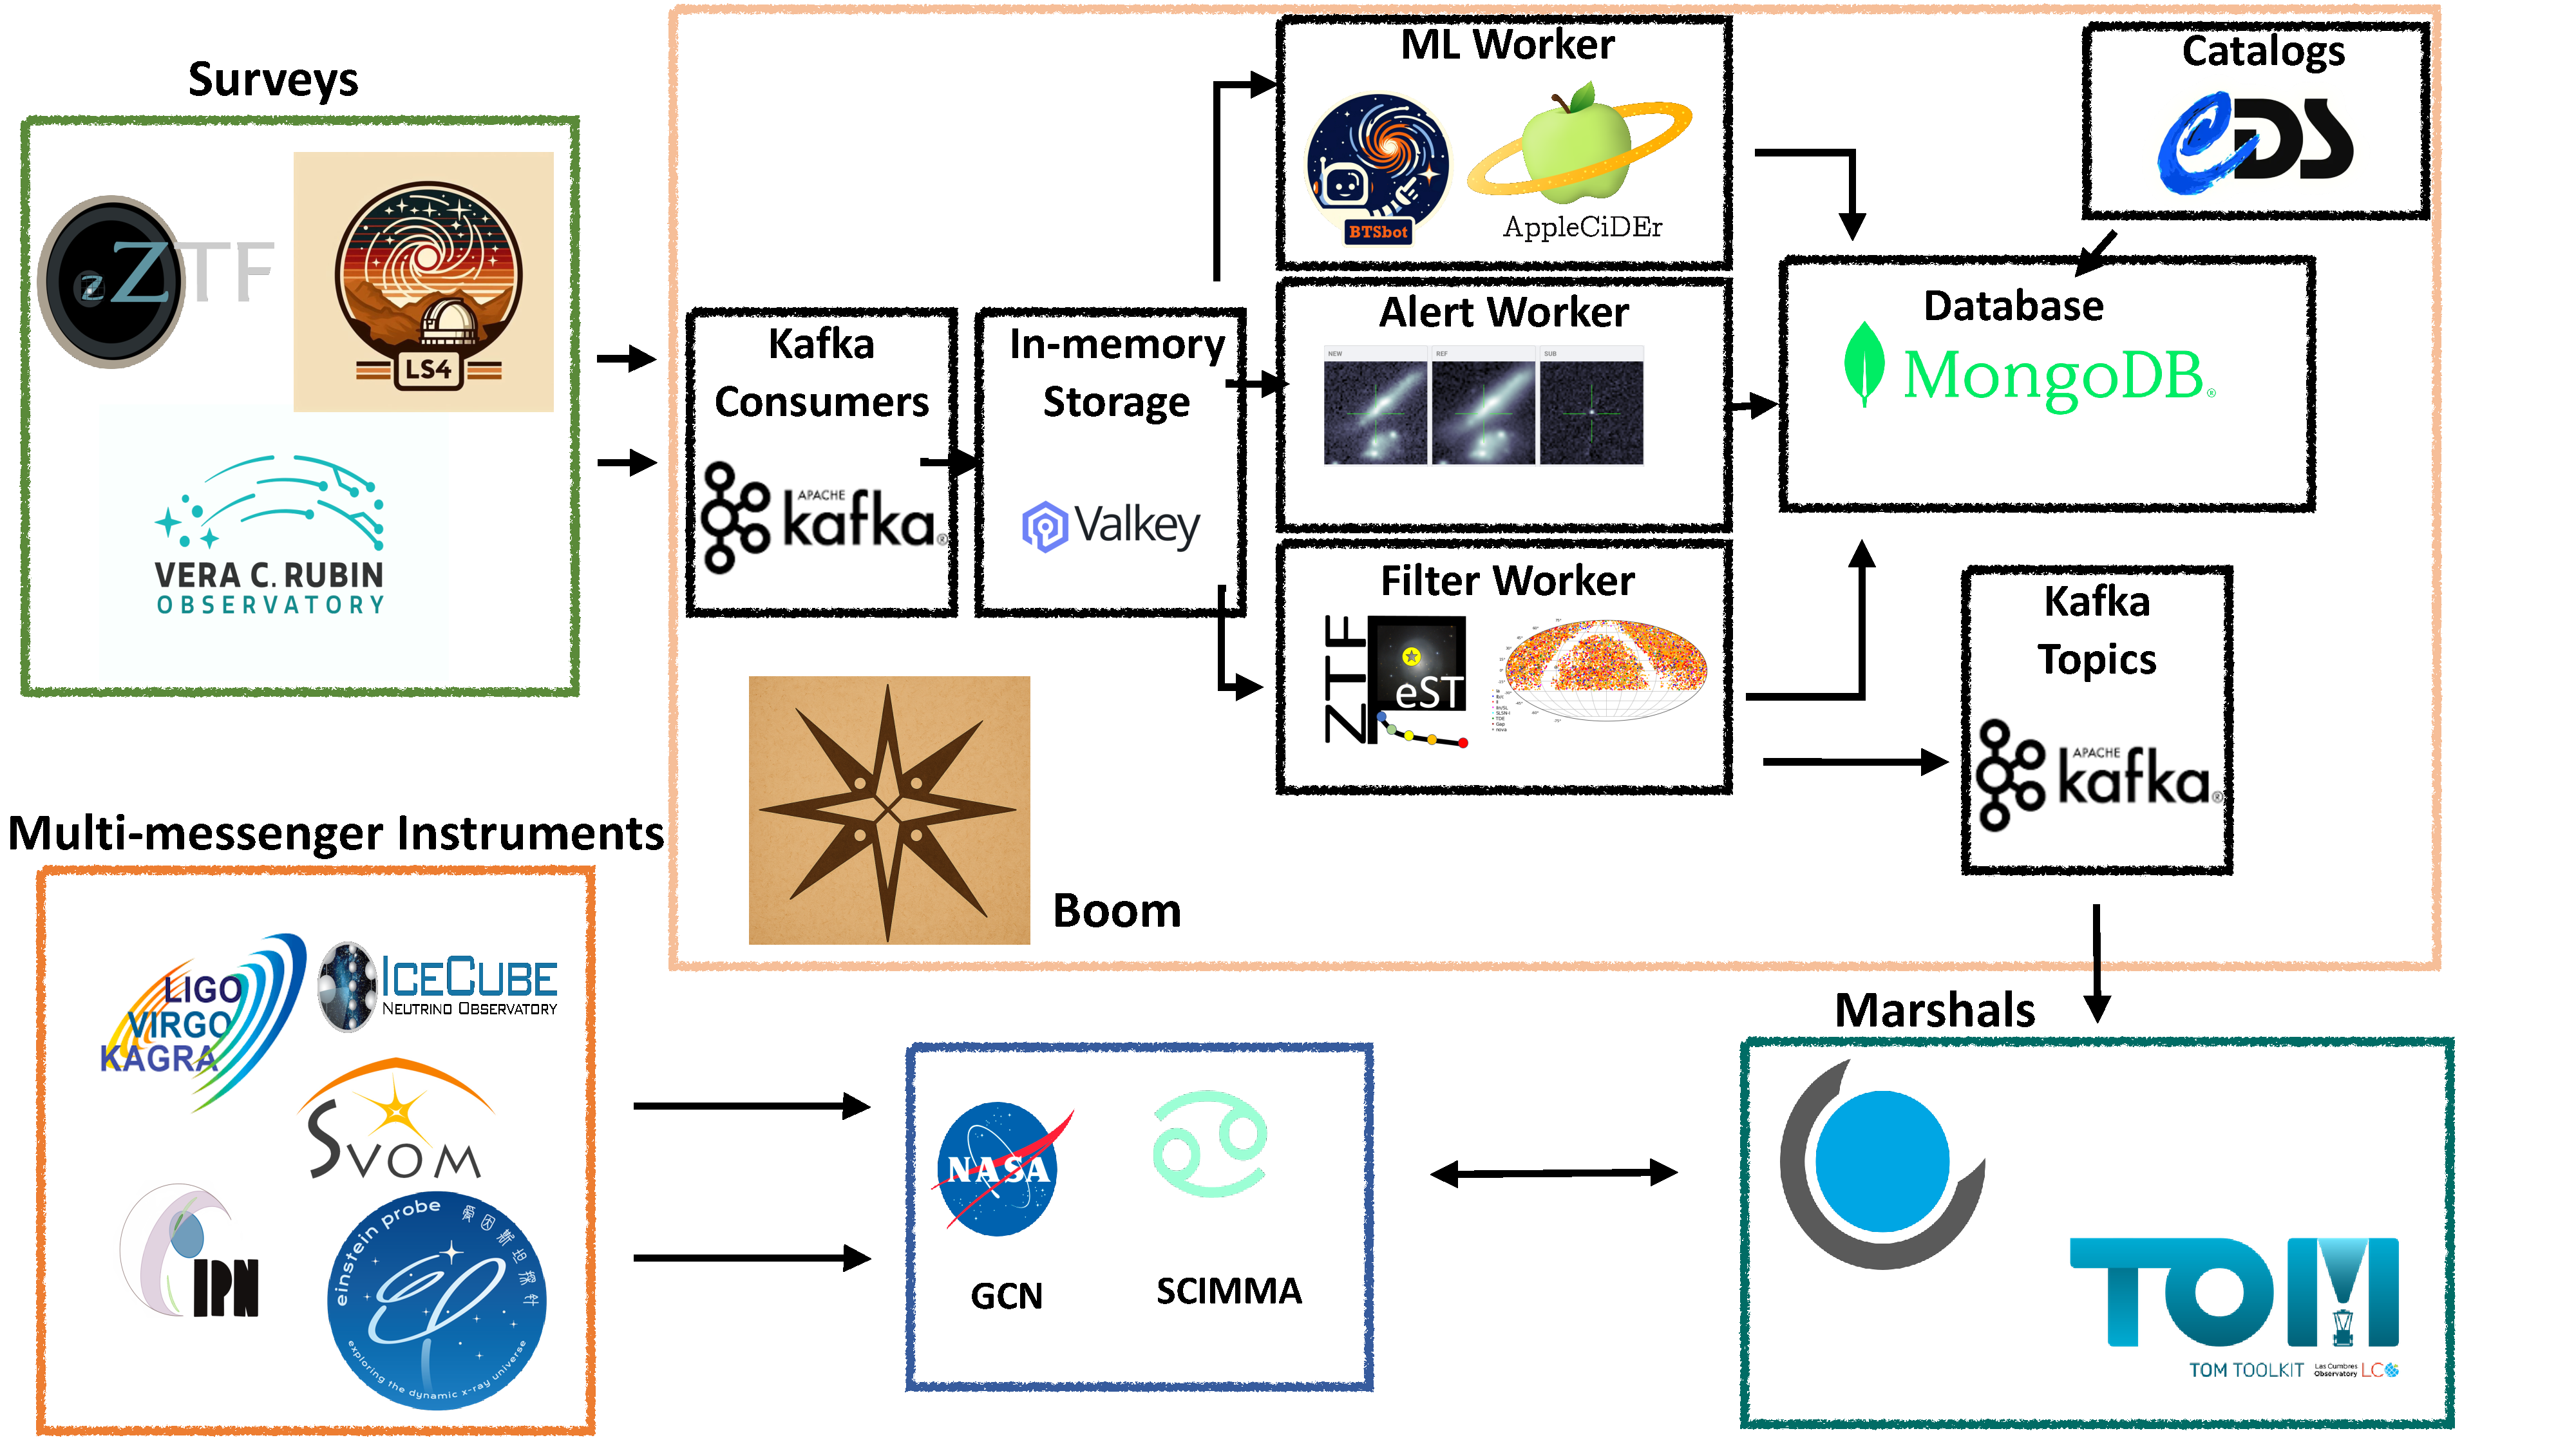
\includegraphics[width=6.5in]{figures/workflow.pdf}
    \caption{Flowchart for BOOM.}
    \label{fig:flowchart}
\end{figure*}

In the following subsections, we present the key design features and implemented capabilities within \texttt{BOOM}.
\texttt{BOOM} is designed for full parallelization. The database and alert processors all scale horizontally, allowing additional workers to be added at any stage to accommodate changes in workload. Alerts can be processed in any order, meaning they do not need to follow a strict time sequence.
\texttt{BOOM} operates with workers, separating the machine learning, cross-matching, filtering, ingestion, etc. into different processes. Each of these workers are described herein.

\subsection{Apache \texttt{Kafka}}

Optical alerts are transmitted as Avro packets\footnote{\url{https://avro.apache.org}}, which contain associated image stamps, metadata, and historical detection information, as detailed in \url{https://zwickytransientfacility.github.io/ztf-avro-alert/schema.html}. To receive alert streams, BOOM utilizes Apache Kafka\footnote{\url{https://kafka.apache.org}}, which also facilitates communication between different pipeline steps via independent Kafka topics.

\texttt{BOOM} employs \texttt{Kafka} consumers for handling the ingestion of transient alerts from astronomical surveys. These consumers listen to Kafka topics where alerts are streamed in real-time, retrieving the data and pushing it into \texttt{Redis}/\texttt{Valkey} queues for further processing. The design allows multiple consumers to operate simultaneously, ensuring high-throughput.

\rednote{Describe how we regulate ingestion}
\rednote{Parallelization with Kafka partitions}

The \texttt{Redis}/\texttt{Valkey} queues serve as an intermediary in-memory storage layer to manage the flow of transient alert data between Kafka consumers and downstream processing workers. By acting as a buffer, \texttt{Redis}/\texttt{Valkey} allows Kafka consumers to quickly offload alerts without waiting for processing to complete, reducing bottlenecks in the ingestion pipeline. Its in-memory operation ensures low-latency retrieval, enabling fast access for the alert ingestion, machine learning, and filtering units. Additionally, it helps prevent \texttt{MongoDB} overload by temporarily holding alerts before they are enriched and stored, mitigating the risk of overwhelming the database during high alert volumes. The queue structure also facilitates parallel processing, allowing different processing units—such as machine learning classifiers and cross-matching services—to consume alerts independently.
\rednote{Memory considerations?}
\rednote{Wait mechanism?}

\texttt{Kafka} is currently the standard for astronomical alert brokering due to its scalability, fault tolerance, and capacity to handle large data volumes. Additionally, its ecosystem of tools and libraries provides a foundation for building the broader system. While \texttt{Redis}/\texttt{Valkey} could have been used as a message broker, adopting \texttt{Kafka} ensures compatibility with existing downstream services, which are designed to consume alerts from \texttt{Kafka} topics. Maintaining a custom messaging solution would have introduced unnecessary complexity. By utilizing \texttt{Kafka} for external message brokering and \texttt{Redis}/\texttt{Valkey} for internal caching and task queuing, \texttt{BOOM} maintains a clear separation between its public-facing alert distribution and internal data processing workflows, optimizing both performance and interoperability.

To evaluate scalability, we tested various Kafka producer configurations simulating an LSST-like data stream. Our results show that our Kafka cluster can ingest all topics at \rednote{XXXXX} MB/s, approximately \rednote{XXXXX} times faster than the anticipated LSST average alert production rate.

\subsection{\texttt{MongoDB} and filters}

\texttt{MongoDB} has proven to be a highly effective choice for alert brokering, as demonstrated by its successful implementation in \texttt{Kowalski}. Its cross-language support, flexibility, and powerful query language make it well-suited for building complex filtering pipelines for transient alerts. Additionally, \texttt{MongoDB} offers both performance and scalability, essential for handling large data volumes efficiently. While \texttt{PostgreSQL} was a potential alternative, it would have required schema enforcement, limiting adaptability in an alert stream where fields can vary significantly. Moreover, \texttt{PostgreSQL} would have necessitated database migrations whenever a new astronomical catalog was integrated for crossmatching. By contrast, \texttt{MongoDB}'s schema-free design allows \texttt{BOOM} to dynamically accommodate new data sources without modifying the database structure, ensuring a more adaptable and maintainable system for real-time alert processing.

The alert ingestion workers are responsible for processing and enriching transient alerts after they are retrieved from \texttt{Redis}/\texttt{Valkey} queues. These workers handle tasks such as extracting relevant fields, applying filtering criteria, and preparing the alerts for storage in \texttt{MongoDB}. To optimize performance, they are designed to operate in parallel, ensuring that multiple alerts can be processed simultaneously.
As alerts arrive, \texttt{BOOM} stores the original Avro files in \texttt{MongoDB} collections for future analysis. To optimize database size, a selected subset of key fields is extracted and stored directly in the database.

While it is theoretically possible to query \texttt{MongoDB} in a way that directly maps results to Rust structs, as well as to serialize Rust structs when writing data, the \texttt{MongoDB} crate inherently performs serialization and deserialization. However, Rust structs enforce a schema, meaning that fields cannot be dynamically omitted when they are null. This would result in a significant number of null fields being stored in the database, leading to unnecessary data bloat. To address this, \texttt{BOOM} utilizes the bson crate to serialize Rust structs into BSON documents, allowing for a sanitization step where null fields and other unwanted attributes are removed before insertion into MongoDB. When querying the database, results can be retrieved either as BSON documents or deserialized Rust structs, depending on the specific use case and processing requirements.

\rednote{Write about filtering}

\subsection{Catalogs and cross-matching}

A cross-match step runs concurrently with alert ingestion, querying external catalogs to gather additional information on objects of interest. While ZTF alert packets already include data on the nearest cataloged sources from the Solar System, PanSTARRS, and Gaia, \texttt{BOOM} extends this by querying \rednote{XXXXX}

\subsection{Machine learning}

Integrating machine learning models presents challenges due to the predominance of Python-based ML frameworks, which are not easily transferable to Rust. While some models have been successfully converted to ONNX and executed using tch-rs, a Rust wrapper for the LibTorch C++ library, this approach has proven difficult to implement consistently across different systems. To address this, leveraging the \texttt{Redis}/\texttt{Valkey} queues as a caching and task queue mechanism allows the ML models to be executed in Python while maintaining the rest of the pipeline in Rust, ensuring that performance-critical components remain optimized while benefiting from Python’s extensive ML and data processing libraries. This approach is particularly advantageous for the filtering pipeline, where Python’s ecosystem facilitates complex computations that would be cumbersome to implement in Rust. Consequently, \texttt{BOOM} adopts a hybrid programming strategy, utilizing Rust for core performance-sensitive operations and Python for tasks where flexibility outweighs minor performance trade-offs.

\rednote{Write about running BTSBot and ACAI (and some first version of CIDER) in the system?}

\subsection{Integrating multiple alert streams}

Nothing in \texttt{BOOM}'s core design is inherently tied to the ZTF stream -- or even to optical data. The only source-specific components are the Kafka client, which reads the alert stream, which ensure that key variables like coordinates are stored in a uniform format. By using a schema-free database, \texttt{BOOM} can store and process alerts from any data stream.

A more complex challenge is designing analysis units that work across different alert sources. For instance, different optical surveys may use varying conventions for encoding filter information, reference systems, and magnitude uncertainties. Additionally, powerful alert metrics are unique to specific surveys. Until standardized formats are adopted, analysis classes will need to be tailored to each new alert stream.

\section{Deployments, Science Validation and First Results}
\label{sec:science}

\subsection{Hardware Requirements}

\subsection{Throughput Testing}

\subsection{Integration with \texttt{SkyPortal}}

As described above, the purpose of filters implemented in brokers like \texttt{BOOM} is to greatly limit the number of alerts that may correspond to astrophysical phenomena of interest for a given user. This rate limiting is typically a combination of automated filtering (e.g. with ML) and/or human inspection.

We have integrated the output of \texttt{BOOM} filters within \texttt{SkyPortal}, where each filter is organized into a dedicated user ``group.'' While for some configurations all candidates are automatically saved to a group, e.g. for automated triggering of spectroscopic follow-up, many times, users manually vet these alerts through a process known as candidate scanning.

\texttt{SkyPortal} naturally allows for multiple alert streams, and so no substantial changes have been required to allow for scanning.
\rednote{Any specific changes to \texttt{SkyPortal} to manage the multiple alert streams?}
The candidates interface displays contextual image cutouts from ZTF and other relevant surveys, light curves, astrometric and photometric metadata (e.g., coordinates, cross-matches with the Transient Name Server), and direct links to external resources. Users can efficiently review this information to identify sources of genuine astrophysical interest and selectively save them for follow-up.

\subsection{Joint ZTF + DECam program}

The DECam Search for Intermediate Redshift Transients (DESIRT; PI Palmese) is a DECam wide field survey that observes ${\sim}100$ square degrees of sky in current Dark Energy Spectroscopic Instrument (DESI) tiles as part of the larger DECam DESI Transient Survey (2DTS) \citep{palmese_desirt_2022, hall_decam_2025}. DESIRT observes in the $gri$ bands down to a depth of $r\approx23.5$ on a $3$ day cadence with the goal of producing high quality light curves for thousands of extragalactic transients at a $z > 0.2$ or a peak brightness of $r\approx20.5$. As part of the 2DTS experiment, ZTF has also begun observations with a daily cadence of the same fields in the sky, offering intra-night observations at an even greater cadence.

DESIRT uses a difference imaging pipeline developed in \citet{hu_image_2022} that utilizes graphic processing units (GPUs) to quickly produce transient alerts. A real-bogus convolution neural net is used to remove artifacts. Finally, all known stars are removed through a Gaia cross match \citep{vallenari_gaia_2023} and the remaining transinents manually reviewed and the interesting alerts are publicly reported on TNS. This program offers a unique prelude to the issues of matching alert streams between a relatively smaller telescope such as ZTF and larger telescope like LSST. The observational depth of DESIRT is $\sim$\,3\,mag deeper than ZTF, comparable to the $\sim$\,4\,mag difference LSST will have.

To test \texttt{BOOM}'s abilities to handle alert streams with vastly different depths, a Kafka stream with ZTF-styled avro alerts was developed, and all nights of observations since the restart of DESIRT in February 2025 have been imported into \texttt{BOOM} and \rednote{I think this is where y'all take over with the results of the alerts}

\section{Conclusions}
\label{sec:conclusion}

The data processing system we have described -- \texttt{BOOM} -- is now operational and performant for ZTF and is well-positioned to scale to LSST. \texttt{BOOM} is designed not only to deliver real-time filtering of incoming alerts as well as maintain a persistent, queryable archive of all LSST alerts throughout the survey’s operational lifetime. This archive will enable retrospective analyses and is structured to support future batch-processing capabilities, facilitating large-scale, post-facto scientific investigations.


\rednote{Describe vision for \texttt{BABAMUL}}
Using the \texttt{BOOM} codebase, we are preparing a public, production filtering of the LSST alert stream enriched by ZTF alerts, which we call \texttt{BABAMUL}. \texttt{BABAMUL} will provide a number of public streams supporting a variety of science cases through SCiMMA Kafka topics. In this way, \texttt{BABAMUL} will serve as a general-purpose alert broker for the U.S. and international astronomy communities taking advantage of the multiple surveys currently online.

More broadly, \texttt{BOOM} empowers researchers with a flexible, scalable platform that naturally allows for brokering multiple surveys simultaneously, which enables for the extraction of the maximum scientific value from current and future surveys.

In the future, we have a number of critical developments we plan for the platform, mostly focused on facilitating filtering of alerts:

\begin{itemize}
\item \rednote{Thomas: can move this into main section once edited.} \textbf{Filter visualization.} We urgently need tools to facilitate the development of astronomical alert filters, by facilitating knowledge sharing and reusability, while greatly simplifying the design of such filters. These requirements hint at the need for visual tools to compose complex and multi-step pipelines using a graph-like system, where users can build filters using simple drag-and-drop mechanisms, and where each filter can be exported as its own module, to later be reimported as one of the many building blocks of much more complex pipelines. By completely abstracting the underlying -- and often too technical -- query language to run such pipelines on a database with high performance, we hope to redirect the scientists' efforts and attention to the higher-level decision-making and design required to successfully execute their science program.
\item \textbf{Filter validation.} We propose the development of software dedicated to re-running these complex filters after the fact, to validate their capabilities, purity, and to estimate the rates at which we can expect automated ToOs for the targeted follow-up instruments. These tools could easily integrate as part of the filter-building process, enforcing validation before proceeding to submission and real-time operations. This way, any iteration of a given filter would automatically come with associated statistics, building a strong baseline and point of reference as we iterate to improve any survey's results.
\end{itemize}

\begin{acknowledgments}

Based on observations obtained with the Samuel Oschin Telescope 48-inch and the 60-inch Telescope at the Palomar Observatory as part of the Zwicky Transient Facility project. ZTF is supported by the National Science Foundation under Grants No. AST-1440341, AST-2034437, and currently Award AST-2407588. ZTF receives additional funding from the ZTF partnership. Current members include Caltech, USA; Caltech/IPAC, USA; University of Maryland, USA; University of California, Berkeley, USA; University of Wisconsin at Milwaukee, USA; Cornell University, USA; Drexel University, USA; University of North Carolina at Chapel Hill, USA; Institute of Science and Technology, Austria; National Central University, Taiwan, and OKC, University of Stockholm, Sweden. Operations are conducted by Caltech's Optical Observatory (COO), Caltech/IPAC, and the University of Washington at Seattle, USA.


M.W.C. acknowledges support from the National Science Foundation with grant numbers PHY-2117997, PHY-2308862 and PHY-2409481.

\end{acknowledgments}

%%%%%%%%%%%%%%%%%%%% REFERENCES %%%%%%%%%%%%%%%%%%

% The best way to enter references is to use BibTeX:

\bibliographystyle{aasjournal}
\bibliography{references} % if your BibTeX file is called example.bib


\label{lastpage}
\end{document}
